\documentclass[UTF8, 11pt]{article}
\usepackage{amsmath}
\usepackage{amssymb}
\usepackage{bm}
\usepackage{caption}
\usepackage{geometry} % set margins
\usepackage{graphicx} % insert images
\usepackage{hyperref}
\usepackage{listings}
\usepackage{parskip}
\usepackage{url}
\usepackage{xcolor}

\bibliographystyle{plain}
\geometry{margin=2cm}
\newcommand{\mr}{\mathrm}
\newcommand{\mrd}{\mathrm{d}}
\newcommand{\munu}{{\mu \nu}}
\newcommand{\taglabel}[1]{\tag{#1}\label{#1}}
\newcommand{\lp}{\left(}
\newcommand{\rp}{\right)}
\newcommand{\subtt}[1]{\subsection{\texttt{#1}}}
\newenvironment{case}{\begin{equation}\begin{cases}}{\end{cases}\end{equation}}
\pagestyle{plain}
\setlength{\parskip}{\baselineskip}

\lstset{
  language=C++,
  basicstyle=\ttfamily\footnotesize,
  keywordstyle=\color{blue},
  commentstyle=\color{gray},
  stringstyle=\color{red},
  numbers=left,
  numberstyle=\tiny\color{gray},
  stepnumber=1,
  numbersep=10pt,
  backgroundcolor=\color{white},
  showspaces=false,
  showstringspaces=false,
  showtabs=false,
  frame=single,
  tabsize=2,
  captionpos=b,
  breaklines=true,
  breakatwhitespace=false,
  title=\lstname
}

\title{Large High Altitude Air Shower Observatory (LHAASO)}
\author{Chuizheng Kong}
\date{\today}

\begin{document}

\maketitle

The Large High Altitude Air Shower Observatory (LHAASO) is a new generation multi-component facility, functioning as both an operational $\gamma-$ray astronomical observatory and a fully functioning CR (CR) air shower detection complex with multiple techniques measuring various shower components.

\section{Ground-based Facility and Instruments}

LHAASO is located at Mt. Haizi (4410 m ASL, 29° 21’ 27.56” N, 100° 08’ 19.66” E) in Daocheng, Sichuan province, P.R.China\cite{cao2022largehighaltitudeair}. LHAASO consists of 1.3 $\mr{km}^2$ array (KM2A) of electromagnetic particle detectors (ED) and muon detectors (MD), a water Cherenkov detector array (WCDA) with a total active area of 78,000 $\mr{m}^2$, 18 wide field-of-view air Cherenkov telescopes (WFCTA) and a newly proposed electron-neutron detector array (ENDA) covering 10,000 $\mr{m}^2$.

\begin{figure}
\centering
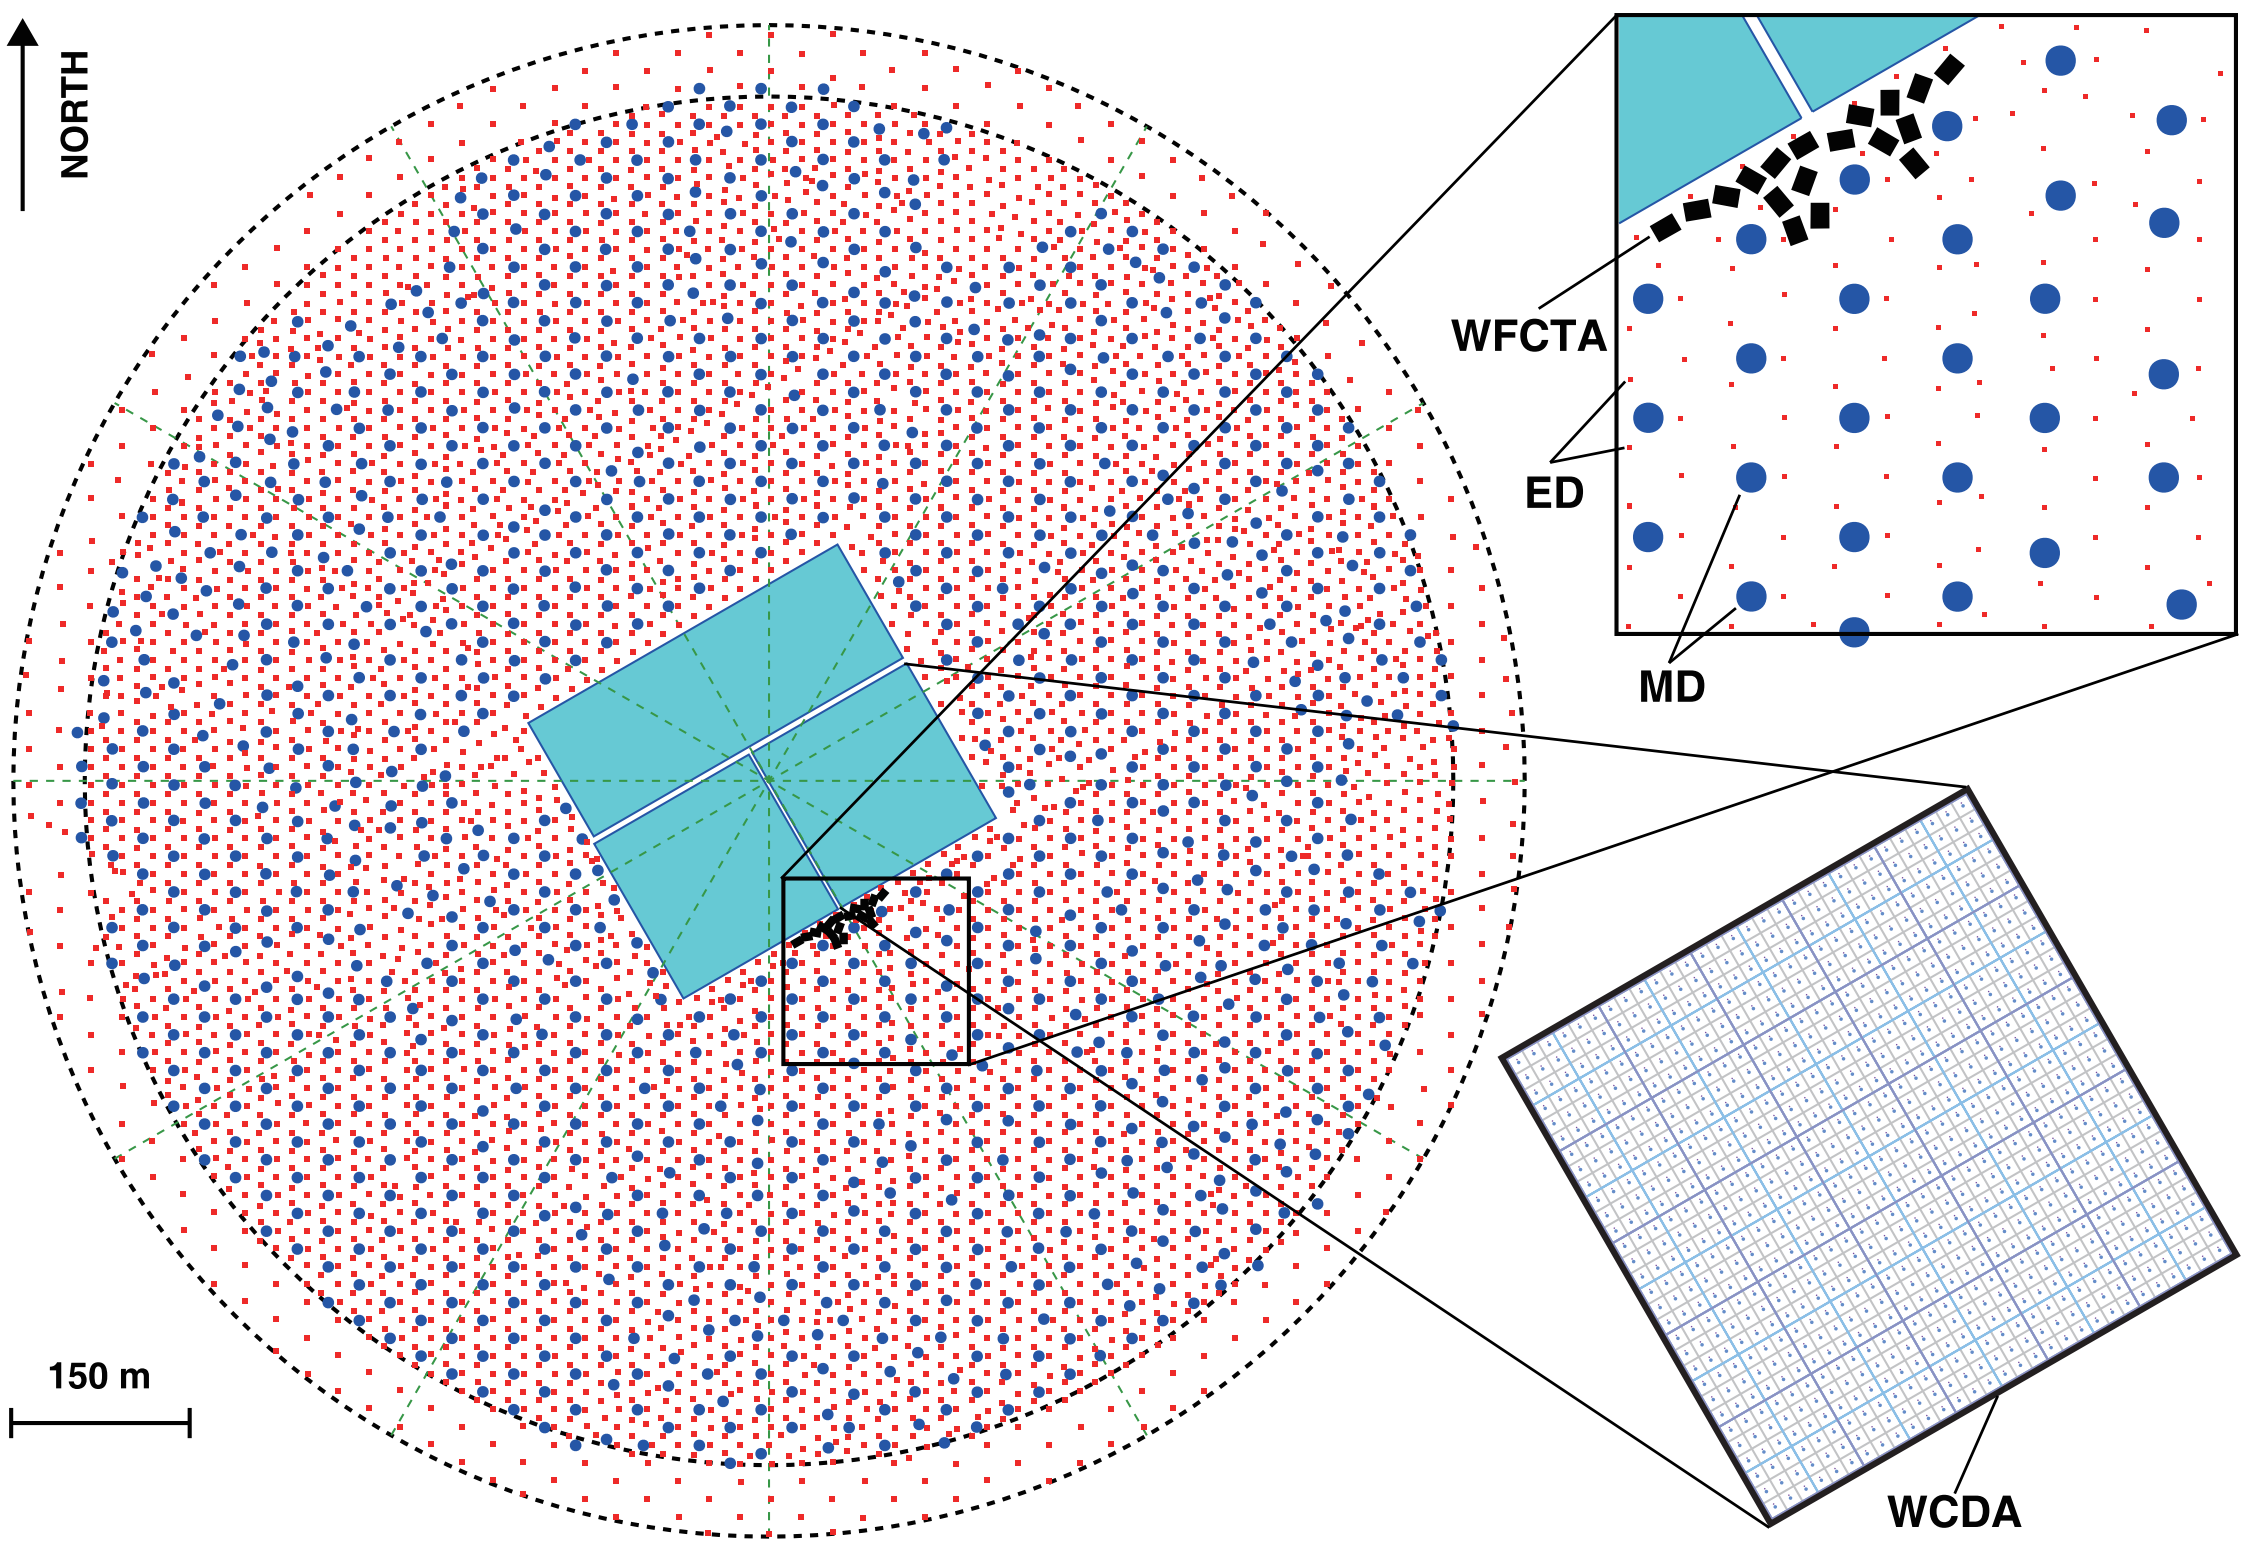
\includegraphics[width=0.7\linewidth]{RPiA/observatory1.png}
\caption{Layout of LHAASO\cite{cao2022largehighaltitudeair}.}
\end{figure}

\section{Messenger Type \& Parameter Space}

LHAASO primarily observes two types of cosmic messengers: CRs and $\gamma-$rays. In more detail\cite{cao2022largehighaltitudeair}, it aims at measuring with unprecedented sensitivity the spectrum, composition and anisotropy of CRs in the energy range between $10^{12}$ and $10^{18}$ eV, and acting simultaneously as a wide aperture continuously-operating $\gamma-$ray telescope in the energy range between $10^{11}$ and $10^{15}$ eV with the designed sensitivity of 1.3\% of the Crab Unit (CU) above 100 TeV.

The KM2A focuses on discovering galactic CR sources by searching for galactic $\gamma-$ray sources above 30 TeV in the northern sky and measuring primary CRs in the energy range from 10 TeV to 100 PeV. WCDA is a survey instrument sensitive to $\gamma-$rays with energies between 100 GeV - 30 TeV. In the energy region of TeV it can attain the world best survey sensitivity of $<$ 0.1 flux intensity of Crab nebula. Besides observation of Galactic $\gamma-$ray sources, WCDA has the discover potential and is sensitive in monitoring extragalactic variant sources, e.g., GRBs, AGNs.

\section{Mission Timeline}

LHAASO is a current mission\cite{ihep2023}, with its construction of the main part begun in 2017 and completed in 2021. LHAASO's quarter-scale detection device was put into trial operation in April 2019, and its full-scale detection instrument was put into trial operation in July 2021.

\section{Main Science Goals}

LHAASO mainly aims at exploring the origin of high-energy CRs and conducting scientific researches on high energy astrophysical radiation\cite{lhaaso}.

The origin of CRs has been listed as one of the top scientific questions in astrophysics. We are yet to solve the origins of high-energy CRs, thus to find out the mechanism of their production and acceleration. LHAASO’s capability of measuring simultaneously different shower components (electrons, muons, and Cherenkov/fluorescence ligh), will allow it to investigate the origin, acceleration, and propagation of CRs through a measurement of energy spectrum, elemental composition, and anisotropy with unprecedented resolution.

The remarkable sensitivity of LHAASO will also allow important studies of fundamental physics (such as indirect dark matter search, Lorentz invariance violation, quantum gravity) and solar and heliospheric physics\cite{ihep2023}.

\bibliography{refer}

\end{document}
